\documentclass{standalone}
\usepackage{tikz,color}
\begin{document}

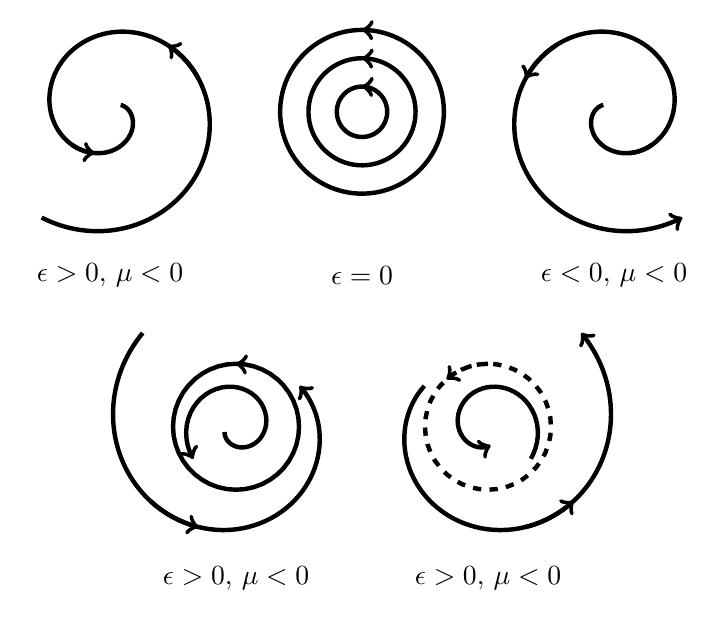
\begin{tikzpicture}[scale=0.8]
\draw [ultra thick, domain=0.2:0.8, samples=100] plot({\x*sin(5*\x r)},{\x*cos(5*\x r)});
\draw [<-, ultra thick, domain=0.7:1.5, samples=100] plot({\x*sin(5*\x r)},{\x*cos(5*\x r)});
\draw [<-, ultra thick, domain=1.4:2, samples=100] plot({\x*sin(5*\x r)},{\x*cos(5*\x r)});
\node at (0,-2.6) {$\epsilon>0,\,\mu<0$};

\draw [<-, ultra thick, domain=0:7, samples=100] plot({0.4*sin(\x r)+4},{0.4*cos(\x r)});
\draw [<-, ultra thick, domain=0:7, samples=100] plot({0.85*sin(\x r)+4},{0.85*cos(\x r)});
\draw [<-, ultra thick, domain=0:7, samples=100] plot({1.3*sin(\x r)+4},{1.3*cos(\x r)});
\node at (4,-2.6) {$\epsilon=0$};

\draw [ultra thick, domain=0.2:0.8, samples=100] plot({8-\x*sin(5*\x r)},{\x*cos(5*\x r)});
\draw [->, ultra thick, domain=0.7:1.5, samples=100] plot({8-\x*sin(5*\x r)},{\x*cos(5*\x r)});
\draw [->, ultra thick, domain=1.4:2, samples=100] plot({8-\x*sin(5*\x r)},{\x*cos(5*\x r)});
\node at (8,-2.6) {$\epsilon<0,\,\mu<0$};


\draw [<-,ultra thick, domain=0.2:0.8, samples=50] plot({2+(1+\x)*sin(5*\x r)},{(1+\x)*cos(5*\x r)-5});
\draw [<-, ultra thick, domain=0.7:1.1, samples=50] plot({2+(1+\x)*sin(5*\x r)},{(1+\x)*cos(5*\x r)-5});
\draw [<-, ultra thick, domain=0:7, samples=50] plot({2+sin(\x r)},{cos(\x r)-5});
\draw [->,ultra thick, domain=0.2:0.85, samples=50] plot({2-\x*sin(10*\x r)},{\x*cos(10*\x r)-5});
\node at (2,-7.4) {$\epsilon>0,\,\mu<0$};


\draw [->,ultra thick, domain=0.2:0.8, samples=50] plot({6-(1+\x)*sin(5*\x r)},{(1+\x)*cos(5*\x r)-5});
\draw [->, ultra thick, domain=0.7:1.1, samples=50] plot({6-(1+\x)*sin(5*\x r)},{(1+\x)*cos(5*\x r)-5});
\draw [->,dashed, ultra thick, domain=0:7, samples=50] plot({6-sin(\x r)},{cos(\x r)-5});
\draw [<-,ultra thick, domain=0.3:0.85, samples=50] plot({6+\x*sin(10*\x r)},{\x*cos(10*\x r)-5});
\node at (6,-7.4) {$\epsilon>0,\,\mu<0$};
\end{tikzpicture}
\end{document}
